
\documentclass[a4paper,twoside, openright, 12pt, leqno]{article}

% Upload template for articles


\usepackage{graphicx}
\usepackage{amsmath, amssymb, bm}
\usepackage{booktabs}

\usepackage{ArticleTemp}

                  % Number theorems
\usepackage{multirow}                    % Multiple rows in tables
\usepackage{placeins}                    % Use \FloatBarrier to put figures and tables in current section

% TABLES: Alignment columns    
\usepackage{array}
\newcolumntype{L}[1]{>{\raggedright\let\newline\\\arraybackslash\hspace{0pt}}m{#1}}
\newcolumntype{C}[1]{>{\centering\let\newline\\\arraybackslash\hspace{0pt}}m{#1}}
\newcolumntype{R}[1]{>{\raggedleft\let\newline\\\arraybackslash\hspace{0pt}}m{#1}}


% Customize headers
\pagestyle{fancy}
\fancyhf{}
\fancyhead[RO,LE]{\small\thepage}
\fancyhead[LO]{\small \nouppercase{FertMort project}}
\fancyhead[RE]{\small \nouppercase{Camarda \& Aburto [Draft]}}
\fancyfoot[L,R,C]{}
\renewcommand{\headrulewidth}{0.4pt}

% Proposition with no numbering
% \newtheorem{proposition}{Proposition}
%\newtheorem*{proposition}{Proposition}
 
% Begin document
\begin{document}

% Remove header from the first page
\thispagestyle{empty}

% Affilations as footnotes with symmbols
% \renewcommand{\thefootnote}{\fnsymbol{footnote}}
\renewcommand{\thefootnote}{\alph{footnote}}

% Hyperlinks in title in black (Except E-Mail address)
\hypersetup{allcolors = black, footnotecolor = black, urlcolor = blue}

\begin{center}
    
    \vspace*{.4cm}
    \LARGE{Forecasting vital rates from demographic summary measures}    
    \vspace{.4cm}
   
    %\hypersetup{footnotecolor=black}
           
   \vspace{1cm}
    \large Giancarlo Camarda\footnote{Institut national d'\'etudes d\'emographiques.  E-Mail: \href{mailto:carlo-giovanni.camarda@ined.fr}{carlo-giovanni.camarda@ined.fr}} and Jos\'e Manuel Aburto\footnote{Interdisciplinary Centre on Population Dynamis University of Southern Denmark \& Max Planck Institute for Demographic Research  E-Mail: \href{mailto:jmaburto@sdu.dk}{jmaburto@sdu.dk}\label{SDU}} 
    %and Fernando Colchero\textsuperscript{\ref{MaxO}}\fnsep\footnote{Department of Mathematics and Computer Science, University of Southern Denmark, Odense, Denmark.}
    
    \vspace{1cm}
    \large\today
    \vspace{1cm}
    
\end{center}

% In text use numbers for footnotes
\renewcommand{\thefootnote}{\arabic{footnote}}
\setcounter{footnote}{0}

% All hyperlinks in blue in text
\hypersetup{allcolors = blue, footnotecolor = blue}

\section*{Abstract}


% Line interpsace
\linespread{1.5}\normalsize
\clearpage

\section{Introduction}
Future levels of mortality and fertility can be predicted by modelling and extrapolating rates over age and time, or by forecasting summary measures of each phenomena and then converted in age-specific rates. For example, in developed countries, the linear increase in life expectancy over some periods has made it easier to fit trends over time of this summary indicator than fitting more complex models based on age-specific dynamics of mortality \citep{White200259}. Therefore, several methods have been proposed to forecast life expectancy. For instance, \citet{torri2012forecasting} forecast life expectancy for a given country assuming a tendency towards a predicted best practice life expectancy. \citet{pascariu2018double} proposed incorporating the analysis of the gap between female and male life expectancy to more accurately predict the overall level of mortality in a country. Similarly, \citet{Raftery2013} forecast life expectancy for several countries using a Bayesian hierarchical model for females, and then model the sex gap to estimate male life expectancy \citep{raftery2014joint}. Subsequently, the overall level of mortality given by life expectancy is converted to a age-specific profile \citep{vsevvcikova2016age}. This latter method has been adopted by the United Nations. However, life expectancy, as an average, conceals the variation in the death distribution \citep{van2018case}. Recently, \citet{bohk2017lifespan} proposed to incorporate the variation in ages at death as an additional indicator to evaluate mortality forecast. This variation is often called lifespan variation or lifespan inequality and refers to how similar ages at death are in a population.
They found that some methods struggle to account for trends in lifespan variation, which results in a mismatch between life expectancy and lifespan variation. In most developed countries, life expectancy and lifespan variation are often negatively correlated \citep{Smits2009,Vaupel2011,colchero2016emergence}, however in some countries this association is less strong, such as Eastern European which might lead to different levels of lifespan variation given a value of life expectancy when forecasted \citep{Aburto2018Eastern}. Therefore, incorporating the dynamics of both life expectancy and lifespan variation to obtain an age-specific mortality profile that matches both is a step forward on more accurately predicting future longevity.

In fertility studies, forecasts usually predict the average number of children that will be born by women over their reproductive lifetime \citep{bohk2018forecast}. Recently, \citet{bohk2018forecast} compared the performance of 20 major methods, including parametric curve fitting methods, extrapolation, Bayesian approaches and context-specific methods, aimed at completing lifetime fertility of women that have not yet reached their last reproductive age. The authors found that more complex methods do not necessarily outperform simpler methods. As in the case of mortality, some of these methodologies rely on modelling age-specific fertility rates (e.g. \citet{coale1974model,chandola1999recent,schmertmann2003system,peristera2007modeling,hyndman2008stochastic}). Others, rely on probabilistic projections of the total fertility rate (TFR). For example, \citet{alkema2011probabilistic} developed a methodology to forecast TFR for all countries using a Bayesian projection model. From these estimates, the age-specific profile can be derived \citep{vsevvcikova2016age}. However, important information in other summary measures such as variance of childbearing age is often ignored \citep{hruschka2016does}.

In this article, we propose a model to obtain future mortality and fertility age-patterns that comply with the projected summary measures. Unlike comparable approaches, we assume only smoothness of future vital rates which is achieved by a two-dimensional $P$-spline approach as in \citet{currie2004smoothing}. Since summary measures are commonly nonlinear functions of the estimated penalized coefficients, Lagrangian multipliers cannot be directly implemented. We hence opted for a Sequential Quadratic Programming (SQP) procedure \citep{nocedal2006sequential} to perform the associated constrained nonlinear optimization. We illustrate our approach with two data sets: mortality of Japanese females, based on future life expectancy predicted by United Nations World Population Prospects \citep{UN2017} and Spanish fertility constrained to total fertility rates, mean and variance of age at childbearing derived by classic time-series analysis.


\section{Model on Japanese mortality data}

For ease of presentation, we formulate the model on mortality data. Suppose that we have deaths, and exposures to risk, arranged in two matrices, 
$\bm{Y} = (y_{ij})$ and $\bm{E} = (e_{ij})$, both with dimension $m \times n_{1}$.  Rows and columns are classified by age at death, $\bm{a}, \,m \times 1$, and year of death, $\bm{t}_{1}, \,n_{1} \times 1$, respectively.  
We assume that the number of deaths $y_{ij}$ at age $i$ in year $j$ is Poisson distributed with mean $\mu_{ij} \,e_{ij}$, where $\mu_{ij}$ is the force of mortality. 
The aim of our model is to reconstruct trends in $\mu_{ij}$ for  $n_{2}$ future years, $\bm{y}_{2}, n_{2} \times 1$ [\textit{This sentence is not completely clear to me}].

\subsection{Life expectancy}

Demographers and actuaries often summarize mortality age-patterns with life expectancy. Life expectancy at birth is the average years a newborn is expected to live given the current mortality rates. In lifetable notation, life expectancy at birth is defined as
\begin{equation*}\label{eq:ex}
e(0)=\int_0^\infty\ell(x)\,dx,
\end{equation*}
where $\ell(x)$ is survival function. Time-trends of this summary measure are often regular and well-understood. Forecasting a single time-series is therefore relatively easy. Figure~\ref{fig:CamardaMort} (left panel) presents observed life expectancy at age 1 for Japanese females from 1960 to 2016 along with the medium variant up to 2050 as computed by the UN. This variant is calculated considering available data for all countries in the world.  The aim of our model is to reconstruct age-specific future mortality patterns that are consistent with this predicted trend.

\begin{figure}[!ht]\centering
	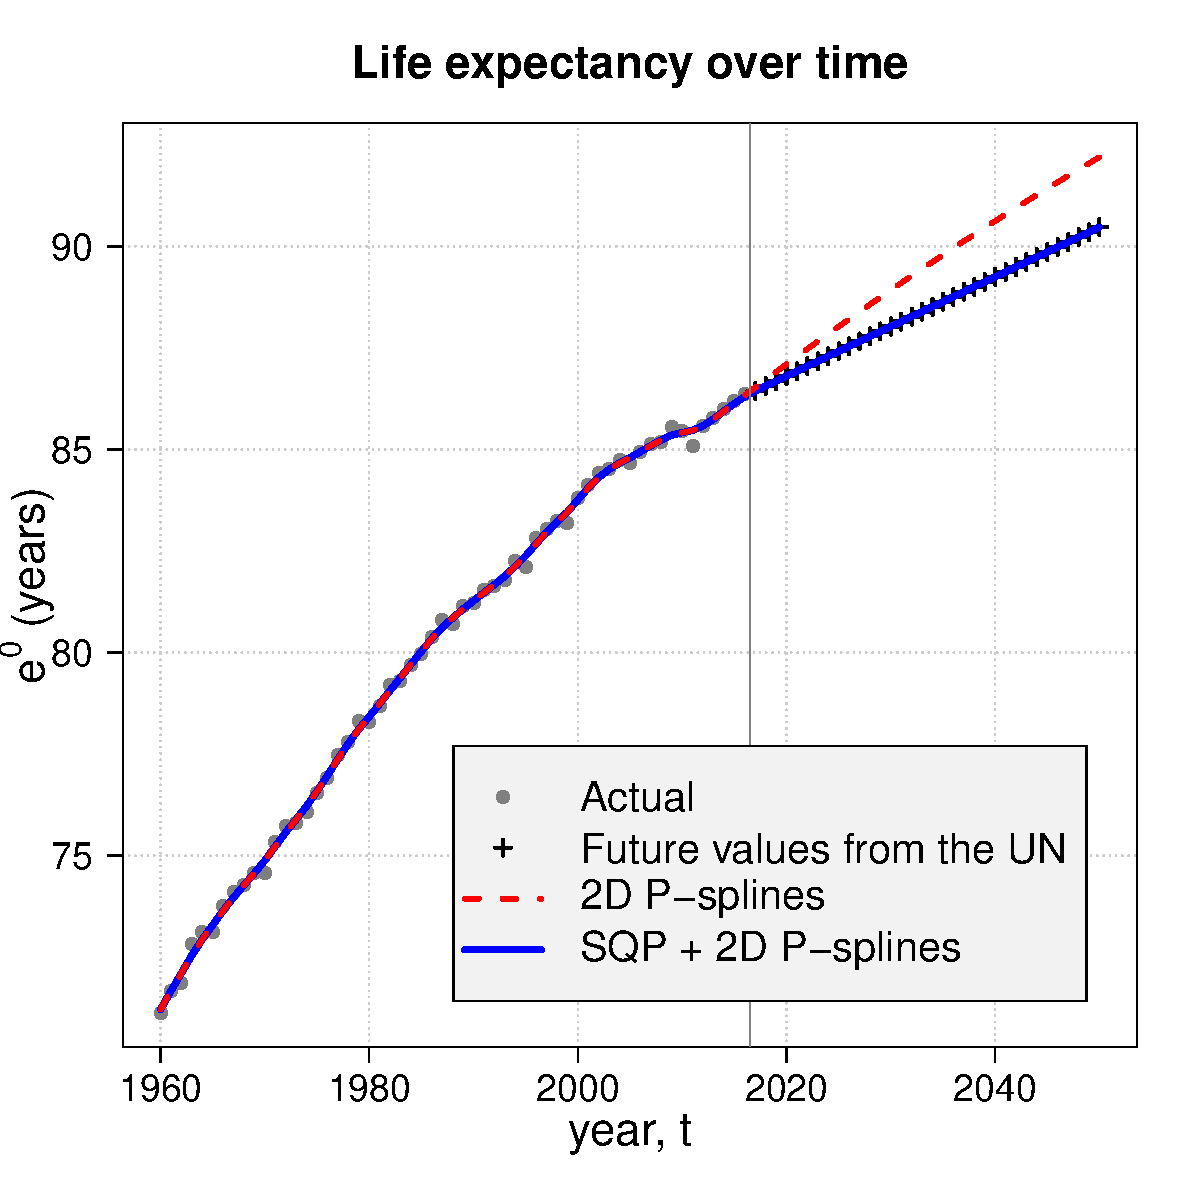
\includegraphics[scale=0.25]{Figures/CamardaE0.pdf}
	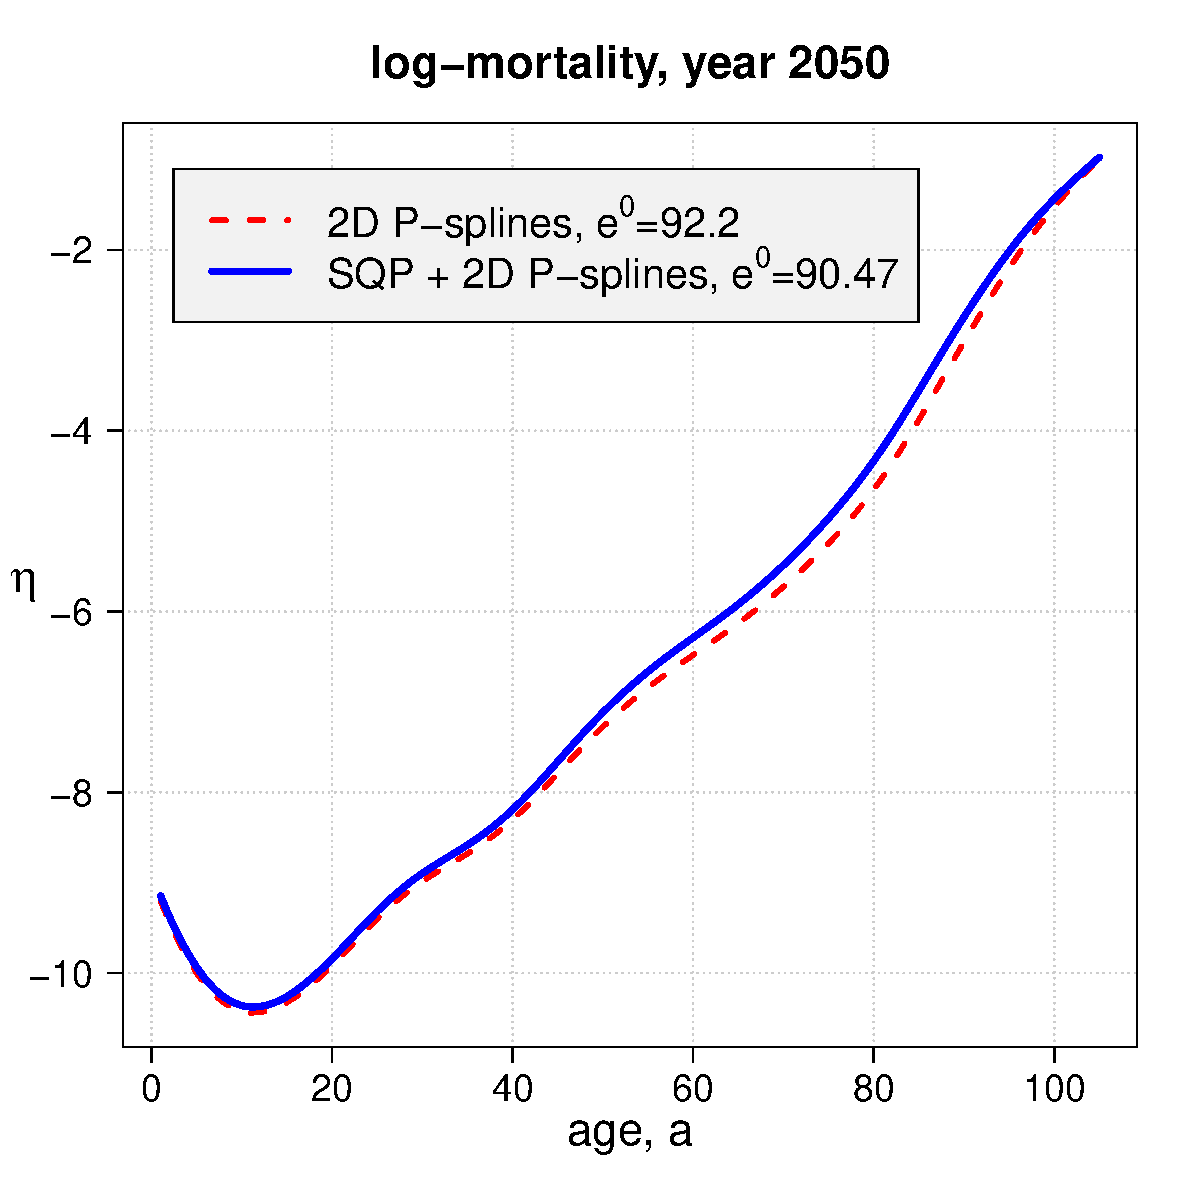
\includegraphics[scale=0.25]{Figures/CamardaMort2050.pdf}
	\caption{\label{fig:CamardaMort} Left panel: Actual, estimated and forecast life expectancy at age 1 by United Nations, 2D $P$-splines and the SQP+2D $P$-splines. Right panel: Mortality age-pattern in 2050 by 2D $P$-splines and the SQP+2D $P$-splines. Japanese females, ages 1-105, years 1960-2016, forecast up to 2050.}
\end{figure}

We arrange data as a column vector, that is, $\bm{y} = \verb"vec"(\bm{Y})$ and $\bm{e} = \verb"vec"(\bm{E})$ and we model our Poisson death counts as follows: $\bm{\eta} = \ln(E(\bm{y})) = \ln(\bm{e})+ \bm{B}\,\bm{\alpha}\, , $ where $\bm{B}$ is the regression matrix over the two dimensions: $\bm{B} = \bm{I}_{n_{1}} \otimes \bm{B}_{a}$, with $\bm{B}_{a} \in \mathbb{R}^{m \times k_{a}}$. Over time, we employ an identity matrix of dimension $n_{1}$ because we will incorporate a constraint for each year. In order to forecast, data and bases are augmented as follows:
\begin{equation}\label{eq:AugData}
\breve{\bm{E}} = [\bm{E} : \bm{E}_{2}]\, , \qquad 
\breve{\bm{Y}} = [\bm{Y} : \bm{Y}_{2}]\, , \qquad
\breve{\bm{B}} = \bm{I}_{n_{1}+n_{2}} \otimes \bm{B}_{a}
\, ,
\end{equation}
where $\bm{E}_{2}$ and $\bm{Y}_{2}$ are filled with arbitrary future values. If we define a weight matrix $\bm{V} = \mathrm{diag}(\verb"vec"(\bm{1}_{m\times n_{1}}:\bm{0}_{m\times n_{2}}))\,$, the coefficients vector $\bm{\alpha}$
can be estimated by a penalised version of the iteratively reweighted least squares algorithm: 
\begin{equation}\label{eq:penIRWLSfor}
(\breve{\bm{B}}^{T} \bm{V} \tilde{\bm{W}} \breve{\bm{B}} + \bm{P}) \tilde{\bm{\alpha}} =
\breve{\bm{B}}^{T}\bm{V} \tilde{\bm{W}}\tilde{\bm{z}} \, ,
\end{equation} 	
where a difference penalty $\bm{P}$ enforces smoothness behaviour of mortality both over age and time. Outcomes from this approach in terms of life expectancy is depicted with a dashed red line in Figure~\ref{fig:CamardaMort} (left panel), and a departure from the UN projected values is evident. 

Note that life expectancy is a nonlinear function of the coefficients vector $\bm{\alpha}$:
\begin{equation}\label{eq:e0}
\bm{e}^{0} (\bm{\alpha}) = (\bm{1}_{1 \times m} \otimes \bm{I}_{n}) \, \exp[ (\bm{I}_{n} \otimes \bm{C}) \verb"vec"(\exp(\bm{B}\bm{\alpha}))]  + 0.5 
\end{equation} 
where $\bm{C}$ is a $(m \times m)$ lower triangular matrix filled only with -1. 
%\begin{equation}\label{eq:Cmat}
%\bm{C} = \left[\begin{array}{rrrr}
%-1 & 0 & \cdots & 0 \\
%-1 & -1& \cdots & 0 \\
%\vdots & \vdots & \ddots & \vdots \\
%-1 & -1 & \cdots & -1
%\end{array}\right] \, .
%\end{equation}  

Constrained nonlinear optimization is therefore necessary and a SQP [\textit{we need to explain more on SQP, perhaps a new subsection}] approach is implemented. Let denote with $\bm{e}^{0}_{\mathrm{T}}$ the $n_{2}$-vector of target life expectancy for future years and with $\bm{N}$ the $(k_{a}n_{2} \times n_{2})$ matrix with derivatives of~\eqref{eq:e0} with respect to $\bm{\alpha}$ for each future year. The solution of the associated system of equations at the step $\nu + 1$ is given by
\begin{equation}\label{eq:SQLalg}
\left[ \begin{array}{l}
\bm{\alpha}_{\nu+1}\\
\bm{\omega}_{\nu+1}
\end{array}\right] = 
\left[ \begin{array}{cl}
\bm{L}_{\nu}& \bm{H}_{\nu}\\
\bm{H}_{\nu}^{T} & \bm{0}_{n_{2} \times n_{2}}
\end{array}\right]^{-1}
\left[ \begin{array}{c}
\bm{r}_{\nu} - \bm{L}_{\nu}\bm{\alpha}_{\nu}\\
\bm{e}^{0}_{\mathrm{T}} - \bm{e}^{0} (\bm{\alpha}_{\nu})
\end{array}\right] \, ,
\end{equation}
where $\bm{L}$ and $\bm{r}$ are left- and right-hand-side of the system in~\eqref{eq:penIRWLSfor}, and matrix $\bm{H}^{T} = \left[\bm{0}_{n_{2}\times k_{a}n_{1}}:\bm{N}^{T}\right]$. Vector of $\bm{\omega}$ denotes the current solution of the associated Lagrangian multipliers.

Forecast $e^{0}$ by the proposed method is exactly equal to the UN values (Figure~\ref{fig:CamardaMort}, left panel). The right panel of Figure~\ref{fig:CamardaMort} shows the forecast mortality age-pattern in 2050: Shape obtained by the suggest approach is not a simple linear function of the plain $P$-splines outcome.

\subsection*{Lifespan variation}

Lifespan variation can be measured with multiple indicators \citep{vanRaalte2013}. These indicators are highly correlated when they measure variation over the full age range, i.e. starting from age 0 \citep{colchero2016emergence}. Here we measure lifespan variation with two indicators: 1) Years of life lost and 2) the Gini coefficient of the life table. 

Years of life lost, denoted with $e^\dagger$, is defined as the average remaining life expectancy when death occurs \citep{Vaupel2003,Vaupel2011}. It is an indicator of absolute variation in lifespans. For example, when death is highly variable, some people will die well before their expected age at death, contributing many lost years to life disparity. When survival is highly concentrated around older ages, the difference between the age at death and the expected remaining years decreases, and life disparity decreases. In life table notation $e^\dagger$ is given by \citep{Goldman1986,Vaupel2003}
\begin{equation*}
e^\dagger = -\int_0^\infty\, \ell(x)\,\ln{\ell(x)}\, dx \,=\, \int_0^\infty\, e(x)\,d(x)\, dx,
\end{equation*}
where $e(x)$ is life expectancy at age $x$, and $d(x)$ is the age-at-death distribution.

The Gini coefficient is an indicator of relative variation. 
\section{Spanish Fertility Data}

We forecast Spanish fertility using three commonly-used summary measures: Total Fertility Rate, mean and variance of childbearing age, forecast by conventional time-series analysis. We then smooth and constrain future fertility age-patterns to comply these forecast values. Summary measures as well as fertility rates in 2050 are presented in Figure~\ref{fig:CamardaFert}. 

\begin{figure}[!ht]\centering
	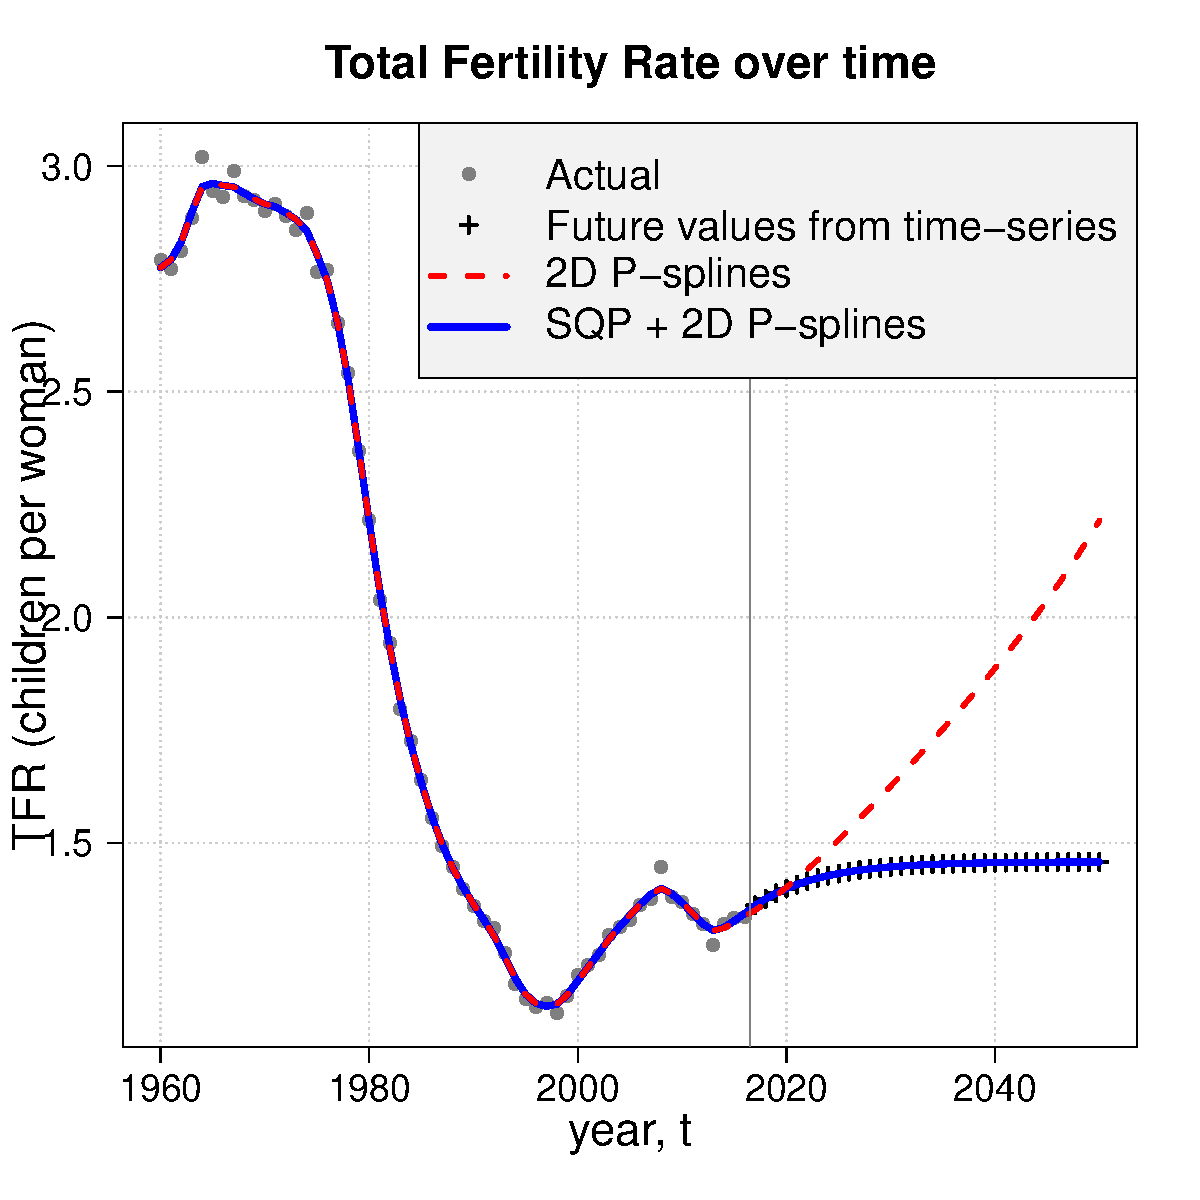
\includegraphics[scale=0.25]{Figures/CamardaTFR.pdf}
	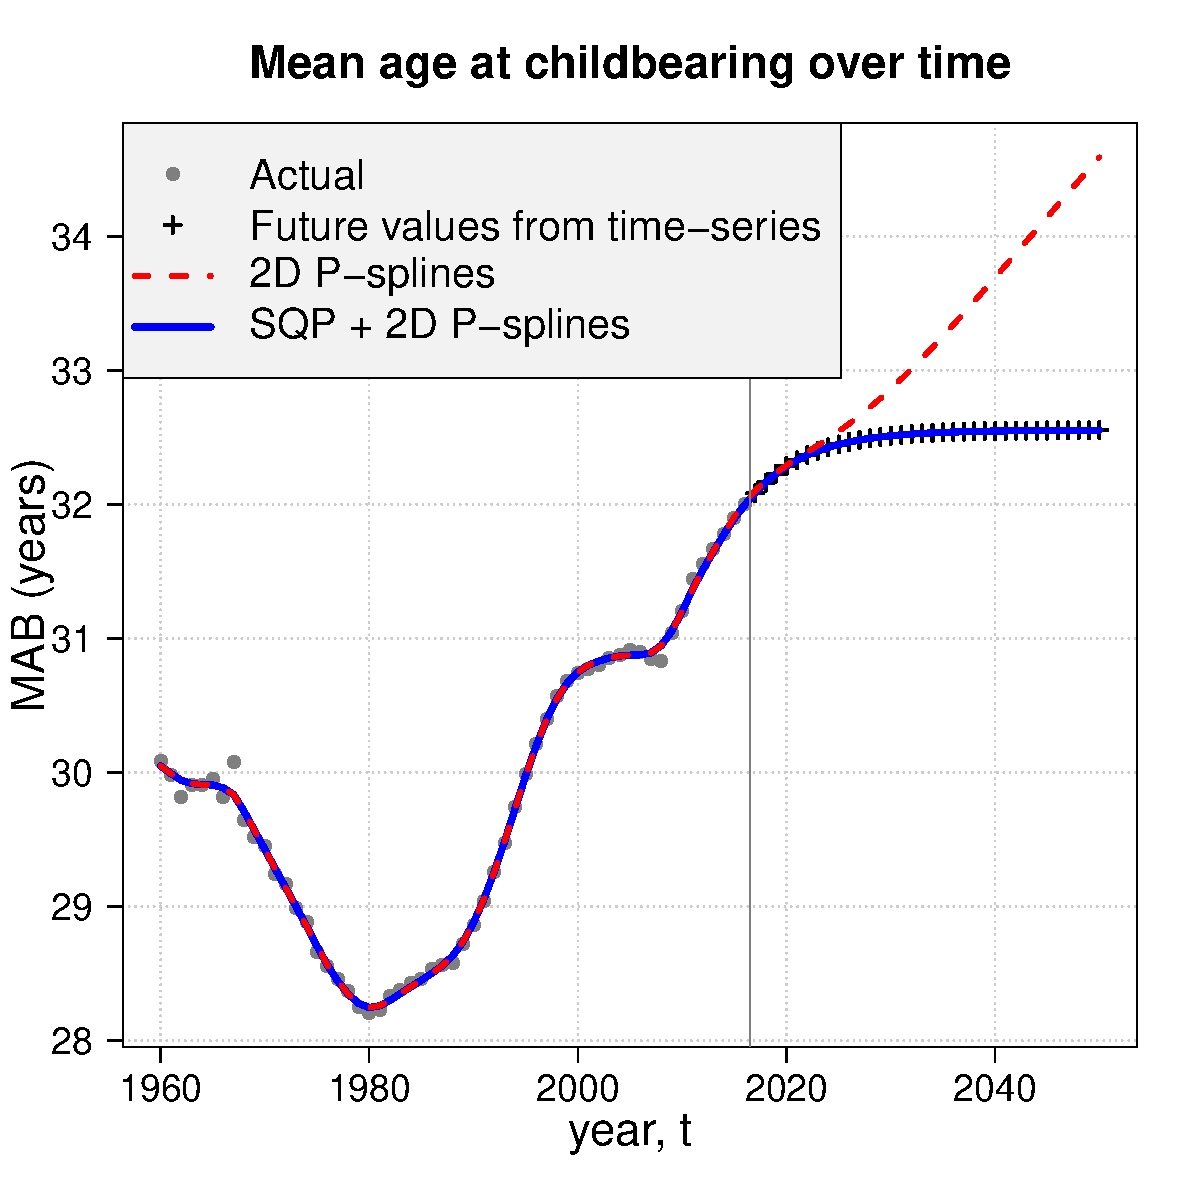
\includegraphics[scale=0.25]{Figures/CamardaMAB.pdf}
	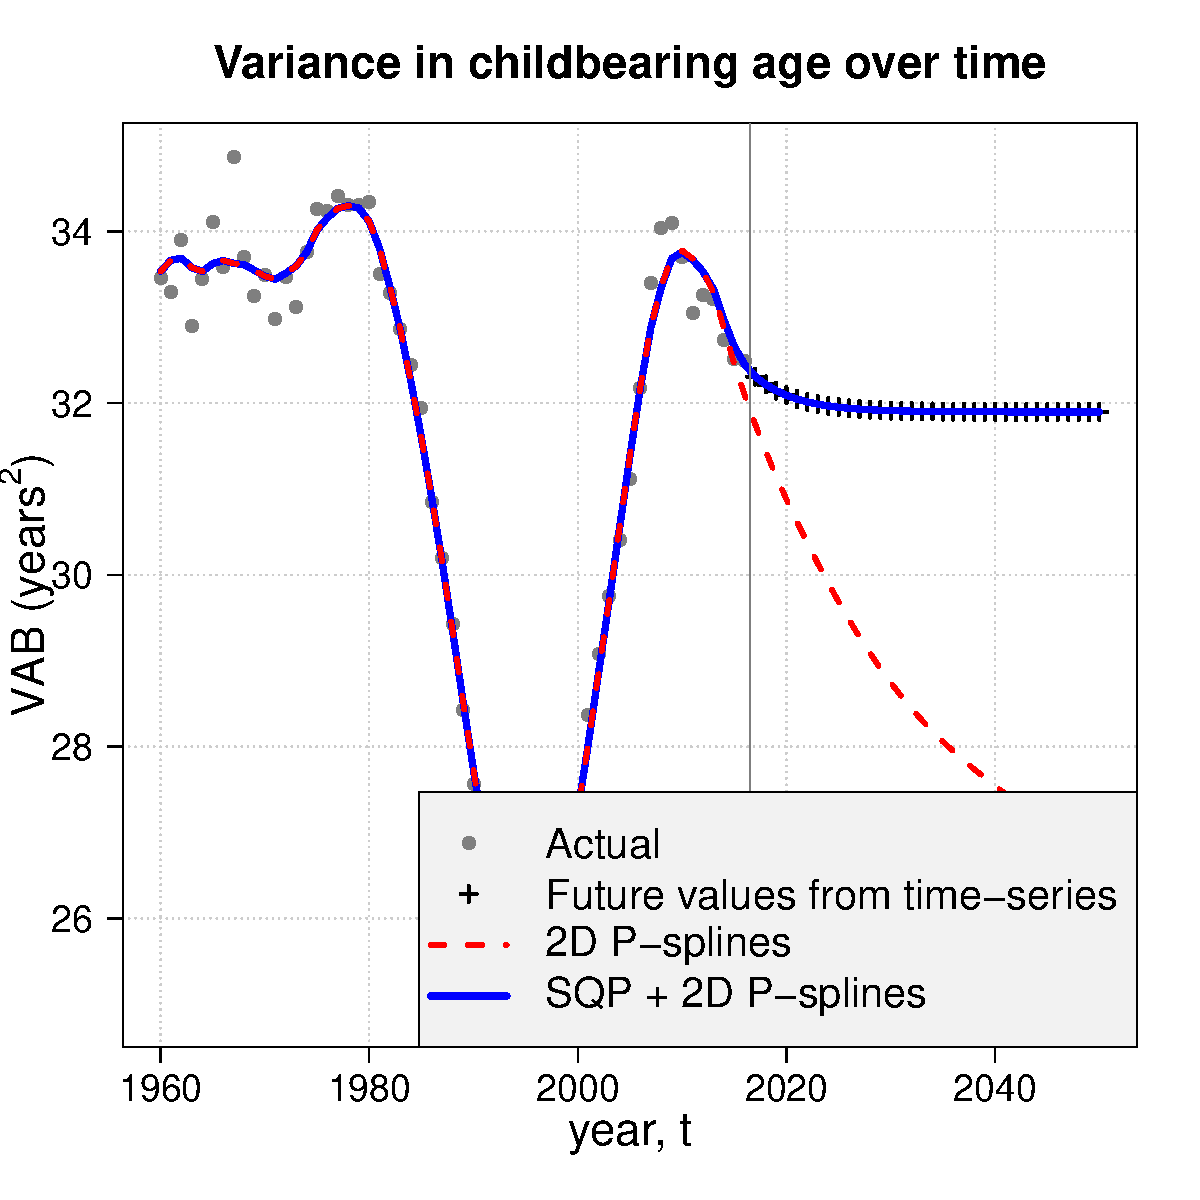
\includegraphics[scale=0.25]{Figures/CamardaVAB.pdf}
	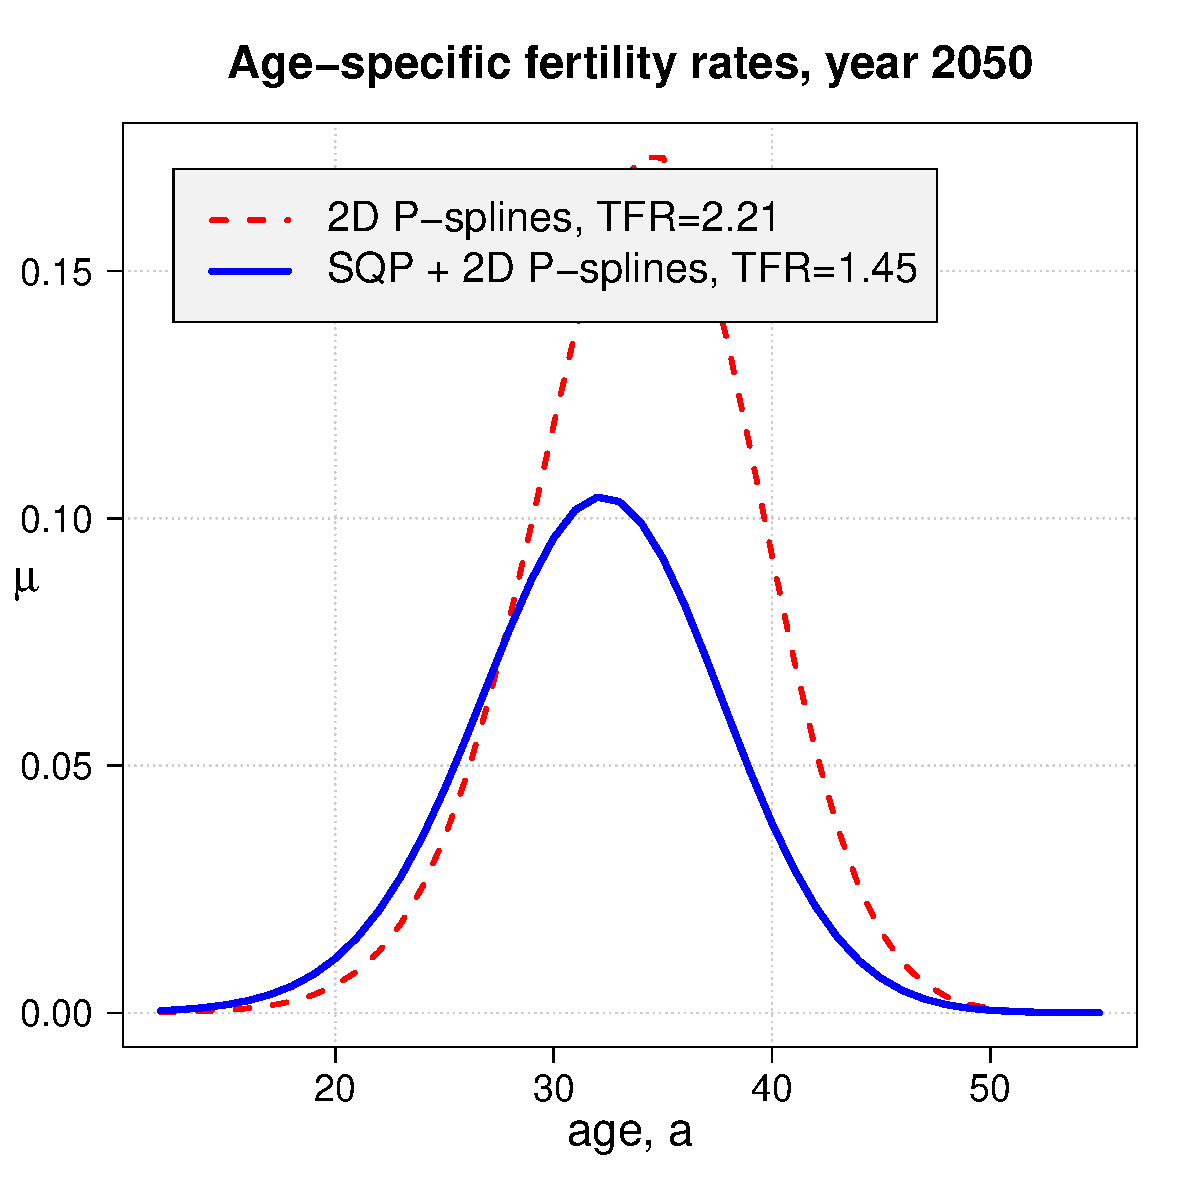
\includegraphics[scale=0.25]{Figures/CamardaFert2050.pdf}
	\caption{\label{fig:CamardaFert} Top and left-bottom panels: Actual, estimated and forecast Total Fertility Rate, Mean and Variance in childbearing age by time-series analysis, 2D $P$-splines and the SQP+2D $P$-splines. Right-bottom panel: Age-specific fertility rate in 2050 by 2D $P$-splines and the SQP+2D $P$-splines. Spain, ages 12-55, years 1960-2016, forecast up to 2050.}
\end{figure}


\section{Discussion}




\section*{Appendix A}

R code 

% Line interpsace
\linespread{1}\normalsize

% Font size
\small

% References
\bibliographystyle{chicago}
\bibliography{Bib_FertMort}

\end{document} 

